\documentclass[a4paper]{article}

\usepackage[T2A]{fontenc}
\usepackage[russian]{babel}
\usepackage{graphicx}
\usepackage{float}
\usepackage{hyperref}
\usepackage{amsmath, amssymb}
\usepackage{caption}
\usepackage{geometry}
\usepackage{pdfpages}
\geometry{top=2cm,bottom=2cm,left=2cm,right=2cm}

\newcommand{\minus}{\scalebox{0.75}[1.0]{$-$}}




\begin{document}

\begin{center}
\textsc{Санкт-Петербургский национальный исследовательский институт информационных технологий, механики и оптики\\[3mm]
Физический факультет} \\[3mm]

\end{center}
\vspace{5mm}
\line(1,0){\textwidth}
\begin{center}
\textbf{ЛАБОРАТОРНАЯ РАБОТА №1.07\\}
\textbf{"Изучение движения маятника Максвелла"}
\end{center}
\vspace{2mm}
\line(1,0){\textwidth}
\vspace{5mm}
\begin{minipage}{0.4\textwidth}
    Группа: Z3144 \\
    Студент: Евгений Турчанин\\
    \vspace{1mm}
\end{minipage}
\hfill
\vspace{1mm}
\line(1,0){\textwidth}


\section{\textbf{Цели работы}}
\begin{enumerate}
\item Определение момента инерции твердого тела на основе законов равноускоренного движения
\end{enumerate}

\section{\textbf{Задачи}}
\begin{enumerate}
\item Провести измерения максимальной высоты, на которую поднимется маятник после спуска, и времени, которое потребуется для достижения данного положения
\item Провести расчет момента инерции на основании прямых измерений
\item Провести теоретический расчёт момента инерции
\item Сравнить результаты обработки экспериментальных данных и теоретического расчета
\end{enumerate}

\section{\textbf{Теория}}
Маятник Максвелла состоит из массивного диска (маховика) и относительно тонкой оси. Маятник подвешивается на двух прочных нитях, концы которых закреплены на оси. Для наблюдения за движением маятника нити наматывают симметричным образом на ось. При этом маятник поднимается из нижнего положения на некоторую высоту $h$.
Когда маятник опускается, его потенциальная энергия переходит в кинетическую. В нижней точке, если пренебречь потерями энергии на трение, имеем:

\begin{equation}
    W_v+W_{\omega}+\Delta U=0
\end{equation}

где $\Delta U$ – изменение потенциальной энергии маятника в поле силы тяжести, $W_v$ – кинетическая энергия, связанная с движением центра масс маятника; $\; W_{\omega}$ – кинетическая энергия вращения вокруг оси симметрии.

\begin{figure}[h!]
    \centering
    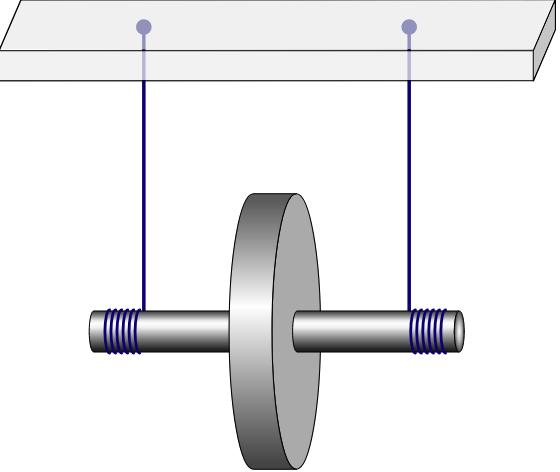
\includegraphics[scale=0.5]{1.png}
    \caption{Общий вид маятника Максвелла}
\end{figure}

Далее из нижней точки маятник за счет своей кинетической
энергии опять поднимется на некоторую высоту $h_1$. Таким образом, в течение некоторого времени его движение будет иметь
квазипериодический характер.\\
Используя известные выражения для энергий $U$, $W_v$ и $W_{\omega}$,
соотношение (1) можно переписать в виде:

\begin{equation}
    mgh=\dfrac{mv^2}{2}+\dfrac{I\omega^2}{2}
\end{equation}



где $m$ – масса маятника, $h$ – начальная высота подъема, $g$ –
ускорение свободного падения, $I$ – момент инерции маятника
относительно оси его вращательного движения, $v$ – скорость в
нижней точке, $\omega$ – угловая скорость в нижней точке. Величина $I$ является аналогом массы при вращательном движении и зависит от распределения массы тела относительно оси вращения.
По причине нерастяжимости нити линейная и угловая скорости связаны соотношением:

\begin{equation}
v=wr
\end{equation}

где $r$ – радиус оси маятника. Полагая, что маятник опускается
с постоянным ускорением $a$, имеем:

\begin{equation}
    v=at; \; h=\dfrac{at^2}{2}
\end{equation}

Отсюда, исключая $a$, получаем

\begin{equation}
    v=\dfrac{2h}{t}
\end{equation}


Подставляя (5) и (3) в (2), находим соотношение для $I$ через измеряемые величины:

\begin{equation}
    I=mr^2\left(\dfrac{gt^2}{2h}-1\right)
\end{equation}


Более строгий подход к определению величины $I$ требует учета потерь энергии в системе за счет трения, а также других причин, в частности, неупругих процессов, связанных с растяжением
нити. Если измерить высоту подъема $h_1$ маятника после однократного опускания, то из закона сохранения энергии имеем:

\begin{equation}
    mgh-mgh_1=M(\varphi-\varphi_1)
\end{equation}


где $M$ – момент сил трения, $\varphi$ и $\varphi_1$ – полные углы поворота маятника при спуске и подъеме


В левой части (7) записана потеря полной энергии за первый
цикл колебаний, а в правой – работа против сил сопротивления
при спуске и подъеме маятника. Тогда (2) следует переписать ввиде

\begin{equation}
    mgh=M\varphi+\dfrac{mv^2}{2}+\dfrac{I\omega^2}{2}
\end{equation}

Учитывая, что:
\begin{equation}
    \dfrac{\varphi}{\varphi_1+\varphi}=\dfrac{h}{h_1+h}
\end{equation}

из (7) находим:

\begin{equation}
    M\varphi=mgh\cdot\dfrac{h-h_1}{h+h_1}
\end{equation}


Подставляя (10) в (8) и используя (3) и (5), получаем более точное, по сравнению с (6) выражение для расчета момента инерции маятника:
\begin{equation}
    I=mr^2\left(\dfrac{gt^2}{h}\cdot\dfrac{h_1}{h+h_1}-1\right)
\end{equation}


\section{\textbf{Экспериментальная установка}}
Схема экспериментальной установки представлена на Рис.2.
\begin{figure}[H]
\centering
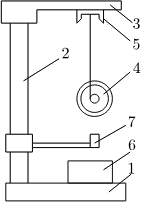
\includegraphics[scale=0.5]{2.png}
\caption{Схема экспериментальной установки}
\end{figure}
\begin{enumerate}
    \item Основание стенда
    \item Опорная колонка
    \item Кронштейн
    \item Маятник Максвелла
    \item Фиксирующий электромагнит
    \item Электронный секундомер
    \item Фотоэлектрический датчик
\end{enumerate}

На основании «1» закреплена колонка «2», на которой находится кронштейн «3», к нему подвешен маятник Максвелла
«4». На кронштейне находится фиксирующий электромагнит «5»,
удерживающий маятник в поднятом положении. Высота подъема
$h$ измеряется по миллиметровой шкале, закрепленной на колонке
«2». Время опускания фиксируется электронным секундомером
«6». При нажатии на кнопку «ПУСК» маятник освобождается, и
одновременно с этим запускается секундомер. Для остановки секундомера в момент прохождения маятником нижнего положения
служит фотоэлектрический датчик «7».
\section{\textbf{Полученные данные}}

\begin{figure}[H]
\centering
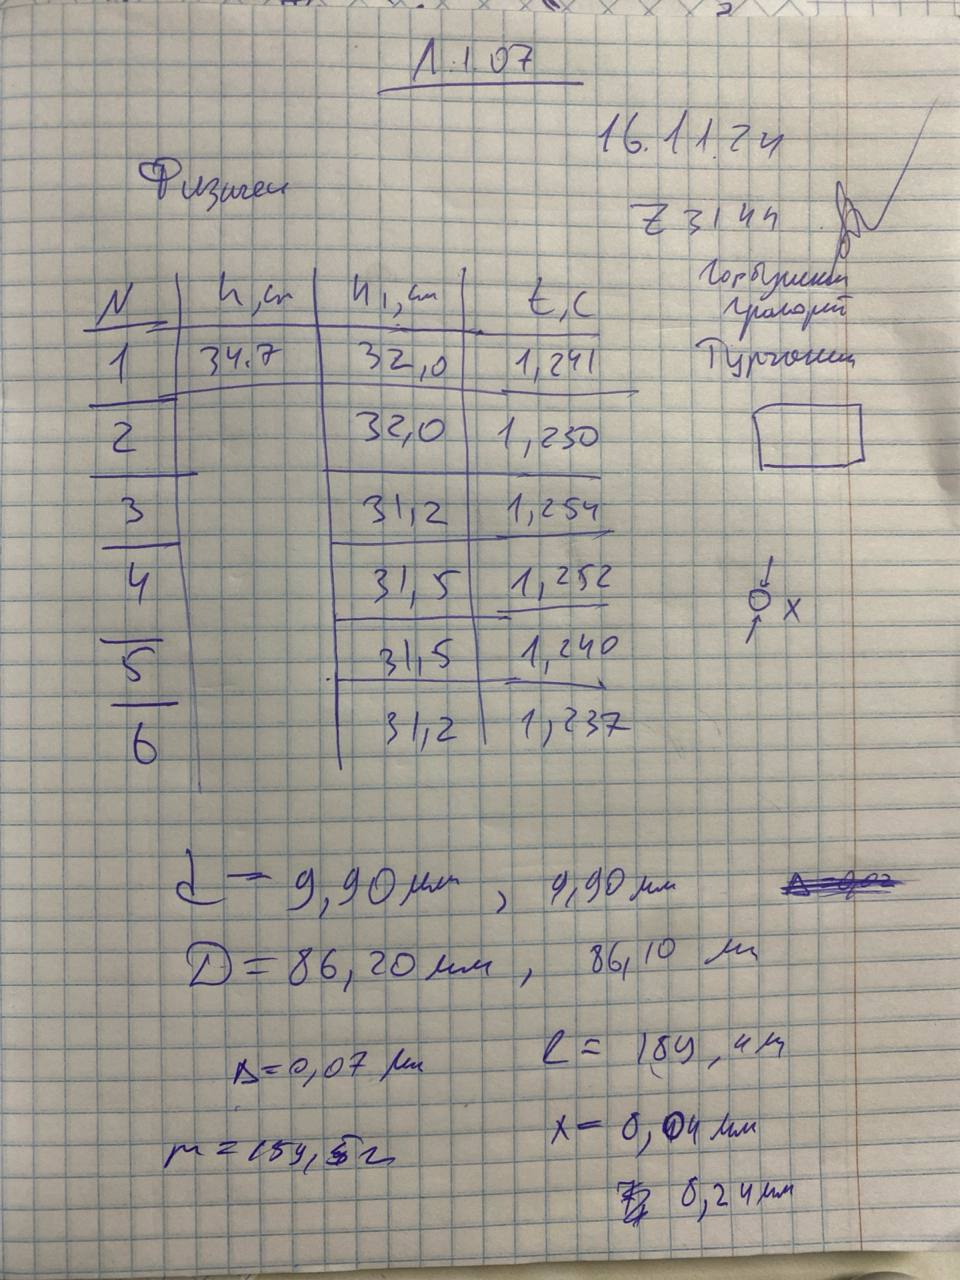
\includegraphics[scale=0.2]{3.png}
\caption{Полученные данные}
\end{figure}


\section{\textbf{Результаты}}




\section{\textbf{Заключение}}




\end{document}
